\section{Alimentação}
	\subsection{Testes e Resultados do Sistema de Inversor}
	
			\begin{figure}[H]
				\begin{center}
					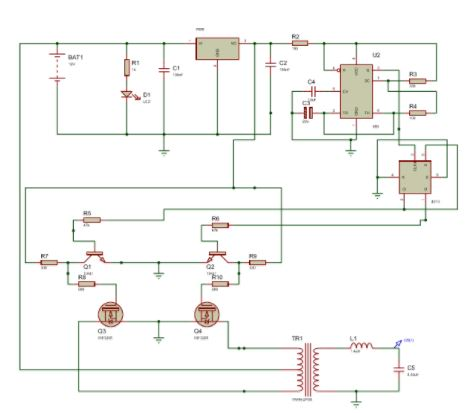
\includegraphics[scale = 0.75]{figuras/Circuito_Inversor}
					\caption{Circuito do inversor simulado no proteus
						}
				\end{center}
			\end{figure}
			
						\begin{figure}[H]
							\begin{center}
								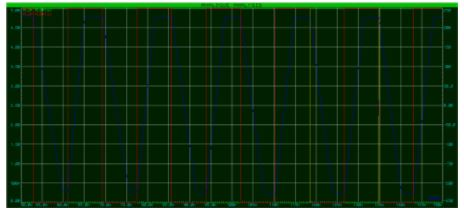
\includegraphics[scale = 0.75]{figuras/Simulacao_Inversor}
								\caption{Circuito do inversor simulado no proteus}
							\end{center}
						\end{figure}

O inversor foi testado inicialmente em um pequeno transformador de 12V para 127 e apresentou uma nível de tensão adequado 127V, porém neste transformador menor não foi ligado a carga pois este não teria capacidade de suportar a tensão com a carga.

Realizamos então o teste com a bateria veícular e o transformador definitivo e o sistema foi capaz de acionar uma lâmpada e cargas menores, com corrente máxima de saída de 0.85A.

\subsection{Outros Testes Realizados}
Foram realizados outros testes com outras topologias de circuito,  porém estes se mostraram insuficientes para o projeto, seja pela carga que este era capaz de suportar ou pela frequência não ser adequada e a sua alta sensibilidade a ruídos externos.

Segue algumas imagens de outros inversores confeccionados, 2 deles foram capazes de acionar a cargade uma lamapada de 40W, mas não foram capazes de realizara partida do motor.

			\begin{figure}[H]
				\begin{center}
				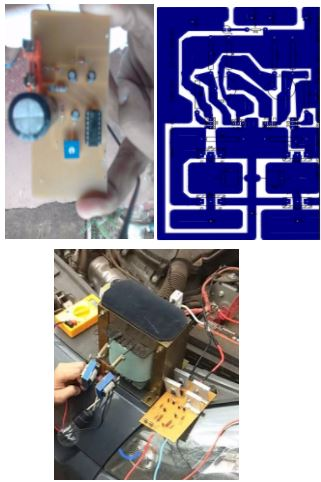
\includegraphics[scale = 0.75]{figuras/Inversor}
				\caption{Layouts e placas de inversor  anteriormente testadas}
				 	\end{center}
			\end{figure}
			
Foram testadas topologias de osciladores com o CI4047 que é um circuito oscilador de onda quadrada ajustável através de um divisor resistivo, porém quando implementado o circuito se mostrou muito instável na frequência de saída, oscilando entre 56Hz e 62Hz, como o CI4047 não possuia modelo de simulação nem no multisim nem no proteus este circuito não foi simulado.

Isso poderia fazer com que os transistores entrassem em curto circuito caso houvesse encontro entre as fases das duas ondas e os testes foram parados para que o banco de potência não fosse danificado.

Também foi testado um circuito com osciladores BC447 e capacitores, que funcionou de com uma frequência próxima de 55 Hz e possuía uma baixa capacidade de fornecer corrente, quando a carga de 40W da lâmpada foi inserida na sua saída, sua tensão abaixou para 114V e a lâmpada ficou vibrando e em luminosidade alta.

Dessa forma o banco de potência  se mostrou insuficiente para gerar a corrente necessária para alimentar a carga.

\subsection{Dificuldades do projeto do inversor}
Durante a confecção e testes do inversor, foram encontradas várias adversidades que dificultaram e atrasaram o processo de fabricação do inversor, a primeira delas é a dificuldade de encontrar componentes eletrônicos para esta aplicação no  mercado brasileiro. Pois, o inversor necessita de componentes de alta potência e baixa dissipação térmica quando há passagem de corrente.

Outra dificuldade foi a falta de um laboratório apropriado para trabalhar com circuitos de alta tensão e circuitos de potência, afinal os osciloscópios da UnB - FGA não dispõem de cabos com atenuadores para que seja possível observar uma forma de onda na saída do inversor.

Além da falta de placas de prototipagem adequadas para circuitos de alta corrente também atrasou o projeto, afinal qualquer teste que fosse feito demandava a elaboração de uma placa de circuito impresso, o que atrasava todo o processo de prototipagem.

Sendo assim, após o estudo e testes dos vários tipos de inversores, evidenciou-se que seria inviável a fabricação de um inversor com o peso conforme os requisitos de projeto e que atendesse as necessidades do sistema, sendo ainda este composto de vários sistemas de proteção e uma corrente estabilizada.

Sendo assim, após o estudo e testes dos vários tipos de inversores, evidenciou-se que seria inviável a fabricação de um inversor com o peso conforme os requisitos de projeto e que atendesse as necessidades do sistema, sendo ainda este composto de vários sistemas de proteção e uma corrente estabilizada.

Seria necessário um maior tempo de estudo e importação de componentes tais como L6386 que é um driver da STD Eletronics próprio para trabalhar altas tensões e temperaturas e com um encapsulamento pequeno e transistores de alta potência para substituir os IRFZ3208 e que possuam uma característica de aquecimento quanto passagem de corrente menor como o transistor IRFP4759BPF, também seria ideal que os componentes do filtro fossem encomendados sob medida para que este ocupe um menor espaço.

Por este motivo foi realizada a compra de um inversor com potência superior ao necessário, como forma de segurança de projeto, para a partida do compressor. A potência necessária para a partida do compressor, já especificada anteriormente é de aproximadamente 1.100W, entretanto foi implementado um modelo de inversor com potência de pico de 3.000 W,  com peso de 2.1 kg.

\subsection{Inversor Implementado}
O inversor implementado é, como demonstrado FIGURA XX, da marca Gilgal com capacidade de transformar uma tensão de 12 V para uma de 220V e capacidade de potência de 3.000 W. Possui características como um botão de liga e desliga, entrada de energia e porta USB. Pode aguentar valores de pico altos de até 3.000W, porém diferente de uma ligação direta, onde existe um pico momentâneo de corrente, esse inversor usa uma ativação soft starter, onde aos poucos chega até a corrente necessária para ativação.	

Diferente de uma ligação direta, que age como um degrau em sua ativação, o soft starter,  faz uma ativação em forma de rampa, o que não exige tanto dos equipamentos em relação ao pico existente, que pode aumentar muito a corrente por alguns segundos e inviabilizar grande parte dos componentes.
			\begin{figure}[H]
				\begin{center}
					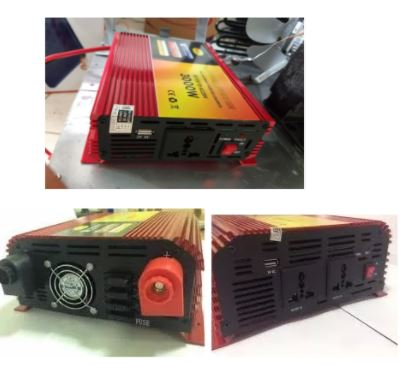
\includegraphics[scale = 0.75]{figuras/Inversor_Implementado}
					\caption{Inversor utilizado no projeto}
				\end{center}
			\end{figure}
\subsection{Testes e Resultados do Sistema de Alimentação}
Para a verificação do funcionamento em conjunto da bateria, inversor, compressor, dissipador e micro motor, alguns testes foram realizados previamente na Faculdade do Gama da UnB, local que a estrutura estava sendo montada. A medição de tensão foi realizada para verificar se atendia ao valor necessário.

			\begin{figure}[H]
				\begin{center}
					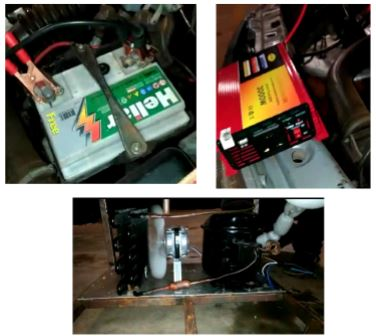
\includegraphics[scale = 0.75]{figuras/Implementacao_Inversor}
					\caption{Teste Sistema de Alimentação Implementado.}
				\end{center}
			\end{figure}
			
Os equipamentos reagiram bem e todos em conjunto, a partida realizada foi em rampa, e não a direta, já que o inversor comprado também possui um soft starter, evitando o problema da alta corrente de pico. Um fator que facilitou a integração com os outros componentes eletrônicos foi também a existência de entrada USB, compatível com parte do material utilizado.

A bateria utilizada, nos testes e implementada no sistema, é da marca Heliar e possui  capacidade de 50A/h, valor que atende a demanda exigida pela transportadora de órgãos. Entretanto, alguns problemas surgiram com o descarregamento desta, fator que causa uma oscilação na alimentação e pode danificar dispositivos mais frágeis, como o GPS. Este problema pode ser resolvido, utilizando uma bateria extra de menor capacidade exclusivamente para o componente.

